\subsubsection{La Vue}
\label{subsubsec:vue}

Chacun des deux modes de jeu possèdent une vue qui lui est propre.
Cela a été rendu possible grâce à plusieurs classes et implémentations.

Pricipalement, nous avons la classe abstraite LabyrinthView.view qui étendue par la classe \textbf{\textit{LabyrinthViewImplementation.java}}, cette classe possède comme attribut d'une instance de \\
\textbf{\textit{LabyrinthPanel.java}} qui est une classe qui étend JPanel et qui est chargée de dessiner le labyrinthe à partir de cellules crées grâce à la classe \textbf{\textit{Cell.java}} qui se basent sur les données du modèle.

Les labyrinthes ont un point de départ et un point d'arrivée que tous les joueurs doivent atteindre.

\newpage

\subsubsection*{Le mode Classique}

La vue du mode classique est gérée par la classe \textbf{\textit{LabyrinthClassicView.java}} qui est une extension de \textbf{\textit{LabyrintheViewImplementation.java}}.

\begin{figure}[!htb]
    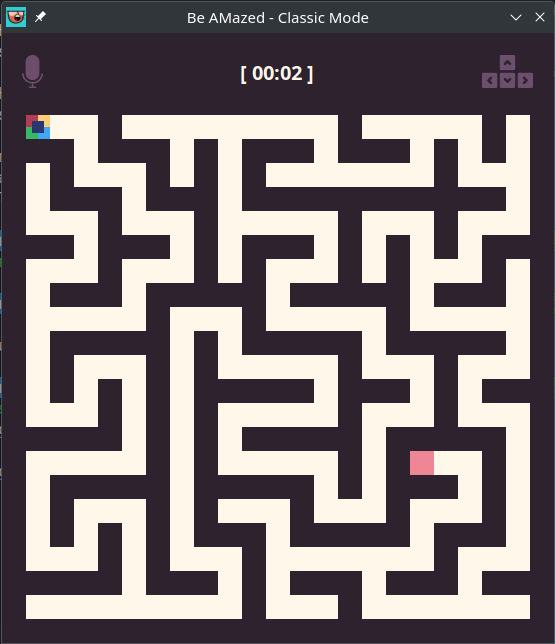
\includegraphics[scale=0.3]{ressources/Implementation/Labyrinthe/Vue/Classic/Classic.png}
    \centering
    \caption{Image du mode Classique}
\end{figure}